% The unit construction (Proposition 7.1).
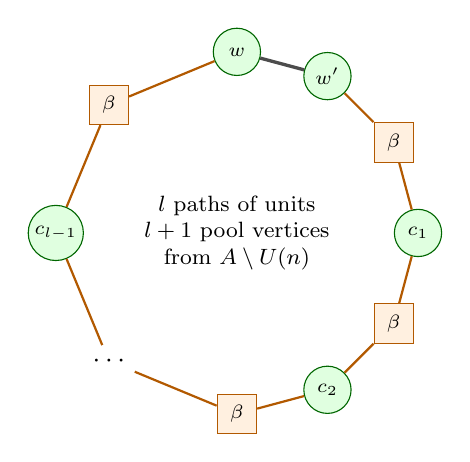
\begin{tikzpicture}[
  un/.style={circle, draw=green!40!black, fill=green!12, inner sep=1.5pt, minimum size=6mm, font=\scriptsize},
  pl/.style={rectangle, draw=orange!70!black, fill=orange!12, inner sep=2pt, minimum size=5mm, font=\scriptsize},
  e/.style={black!70}, j/.style={orange!70!black, thick}]
\def\R{2.3}
\node[un] (w) at (90:\R) {$w$};
\node[un] (w2) at (60:\R) {$w'$};
\node[pl] (b1) at (30:\R) {$\beta$};
\node[un] (c1) at (0:\R) {$c_1$};
\node[pl] (b2) at (-30:\R) {$\beta$};
\node[un] (c2) at (-60:\R) {$c_2$};
\node[pl] (b3) at (-90:\R) {$\beta$};
\node (d) at (-135:\R) {$\cdots$};
\node[un] (cl) at (180:\R) {$c_{l-1}$};
\node[pl] (b4) at (135:\R) {$\beta$};
\draw[e, very thick] (w) -- (w2);
\draw[j] (w2) -- (b1) -- (c1) -- (b2) -- (c2) -- (b3) -- (d) -- (cl) -- (b4) -- (w);
\node[font=\footnotesize, align=center] at (0,0) {$l$ paths of units\\ $l+1$ pool vertices\\ from $A\setminus U(n)$};
\end{tikzpicture}
